% Artículo final, Proyecto MAIA 2026-2, Grupo 7, Fundación Canguro
% Compilar: latexmk -pdf articulo.tex  (o pdflatex dos veces)
\documentclass[conference,letterpaper,10pt]{IEEEtran}
\IEEEoverridecommandlockouts
\usepackage[T1]{fontenc}
\usepackage[utf8]{inputenc}
\usepackage{mathptmx}
\usepackage[letterpaper,margin=2.5cm,columnsep=0.6cm]{geometry}
\usepackage{amsmath,amssymb}
\usepackage{graphicx}
\usepackage{booktabs}
\usepackage{array}
\usepackage{multirow}
\usepackage{cite}
\usepackage{tikz}
\usetikzlibrary{positioning,arrows.meta}
\usepackage{url}
\usepackage{microtype}

% ---- Formato del curso: secciones numeradas 1, 2, 3 en negrita; Figura/Tabla ----
\makeatletter
\def\section{\@startsection{section}{1}{\z@}{2.0ex plus 1ex minus .5ex}%
  {1.0ex plus .5ex}{\normalfont\normalsize\bfseries}}
\def\subsection{\@startsection{subsection}{2}{\z@}{1.5ex plus 1ex minus .5ex}%
  {0.6ex plus .3ex}{\normalfont\normalsize\bfseries}}
\renewcommand\thesection{\arabic{section}}
\renewcommand\thesectiondis{\arabic{section}.}
\renewcommand\thesubsection{\thesection.\arabic{subsection}}
\renewcommand\thesubsectiondis{\thesection.\arabic{subsection}}
\renewcommand\thetable{\arabic{table}}
\makeatother
\renewcommand{\figurename}{Figura}
\renewcommand{\tablename}{Tabla}
\renewcommand{\refname}{Referencias}
\renewcommand{\abstractname}{Resumen}
\renewcommand{\IEEEkeywordsname}{Palabras clave}
\newcommand{\var}[1]{\texttt{\detokenize{#1}}}

\begin{document}

\title{Del nacimiento a los 20 años: ¿anticipa la historia clínica temprana la estructura y la destreza motora de adultos nacidos prematuros? Aprendizaje automático en la cohorte KMC-400}

\author{\IEEEauthorblockN{Andrés Felipe Romero Grajales, Mateo Hernández Gualdrón, María Paula Saa Beltrán,\\ Martín Alejandro Quintero Rincón y Juan Pablo Buriticá Ruiz}
\IEEEauthorblockA{Grupo 7, Proyecto Fundación Canguro\\ Maestría en Inteligencia Artificial, Universidad de los Andes, Bogotá, Colombia\\
\{af.romerog1, m.hernandezg234, m.saa, ma.quinteror1, j.buriticar2\}@uniandes.edu.co}}

\maketitle

\noindent\textbf{Resumen.} La prematurez deja alteraciones cerebrales que persisten en la adultez, pero su relación con el desempeño funcional no es lineal. Con la cohorte del ensayo aleatorizado del Método Madre Canguro reevaluada a los 20 años (KMC-400), estudiamos si la información clínica de los primeros 12 meses permite anticipar la estructura motora cerebral y la destreza manual fina (Nine-Hole Peg Test, NHPT). Comparamos 209 adultos nacidos con menos de 1801~g contra 28 controles a término, definimos una etiqueta normativa de preservación estructural (\emph{hardware OK}) anclada a esos controles y entrenamos modelos con validación cruzada anidada, pruebas de permutación y corrección de Holm, agregando variables en seis etapas del desarrollo. Los prematuros tienen volúmenes motores menores (g de Hedges hasta $-0{,}90$), pero un NHPT similar al de los controles ($g = 0{,}12$). La destreza fina no fue predecible en ninguna etapa ($R^2 \le 0$), y un fenotipo de resiliencia basado en el residual estructura--función tampoco (ROC-AUC 0,52--0,56). La estructura motora sí fue predecible desde el nacimiento (AUC 0,70) hasta los 12 meses (0,77), pero casi toda la señal provino del perímetro cefálico y el sexo; al descontar el volumen intracraneal persistió una señal modesta (AUC 0,64--0,67) no atribuible a variables clínicas específicas. Reportamos estos resultados nulos y parciales como hallazgos, junto con un flujo reproducible y desplegado en la nube.

\vspace{4pt}\noindent\textbf{Palabras clave:} prematurez, Método Madre Canguro, neuroimagen, aprendizaje automático, coordinación motora.


% =====================================================================
\section{Introducción}

En 2019 nacieron en el mundo unos 15,2 millones de niños prematuros, cerca del 11\,\% de los nacidos vivos, y la prematurez explica alrededor de un tercio de las muertes neonatales; las recomendaciones de la OMS de 2022 establecen el Método Madre Canguro (MMC) como cuidado de rutina para todo recién nacido prematuro o de bajo peso \cite{darmstadt2023}. En los sobrevivientes, la prematurez se asocia con alteraciones del neurodesarrollo que persisten hasta la adultez (Sección~2.1). El MMC, que combina contacto piel a piel, lactancia materna y alta temprana con seguimiento, fue evaluado en Bogotá en un ensayo clínico aleatorizado entre 1993 y 1996, y su seguimiento a 20 años mostró efectos protectores duraderos en el entorno familiar, la conducta y el volumen de estructuras cerebrales como el caudado izquierdo \cite{charpak2017,charpak2022}.

La Fundación Canguro plantea una observación clínica que motiva este trabajo: hay adultos nacidos prematuros con alteraciones visibles en la resonancia que rinden con normalidad en pruebas de coordinación, y otros con anatomía conservada que rinden por debajo de lo esperado. El proyecto se propuso estudiar esa disociación entre la estructura cerebral (el \emph{hardware}) y el desempeño motor (el \emph{software}) a los 20 años, y preguntarse qué características de la historia clínica temprana la explican.

Los objetivos fueron: (i) caracterizar la estructura motora cerebral y la destreza manual fina de los adultos nacidos con menos de 1801~g frente a controles a término; (ii) evaluar si las variables clínicas del primer año permiten predecir el desempeño motor, la preservación de la estructura motora o un fenotipo de resiliencia, y desde qué etapa; y (iii) entregar el análisis como un flujo reproducible, con un tablero de resultados poblacionales desplegado en la nube.

Las contribuciones son tres. Primero, un resultado negativo bien sustentado: con validación anidada, permutaciones y corrección por multiplicidad, ni la destreza fina ni un fenotipo de resiliencia son predecibles con la información temprana. Segundo, una etiqueta normativa de preservación estructural anclada a controles a término, con un análisis prerregistrado que separa el \emph{tamaño} de la \emph{calidad} de la estructura. Tercero, un sistema de ingeniería reproducible (datos versionados, 42 decisiones documentadas, integración continua y despliegue). La Sección~2 revisa el estado del arte, la Sección~3 describe la metodología, la Sección~4 presenta los resultados, la Sección~5 los discute y la Sección~6 concluye.

% =====================================================================
\section{Estado del arte}

\subsection{Prematurez y cerebro adulto}
Volpe describe la lesión cerebral del prematuro como una combinación de daño destructivo y alteración del desarrollo que compromete la sustancia blanca, los ganglios basales, el tálamo y el cerebelo \cite{volpe2009}. Estos cambios persisten: en adultos jóvenes nacidos muy prematuros se reportan menores volúmenes de sustancia gris y alteraciones de la sustancia blanca asociadas a la edad gestacional y al desempeño cognitivo \cite{nosarti2014}. En difusión, la interpretación no es directa: Groeschel et al. encontraron en adolescentes prematuros una anisotropía fraccional (FA) \emph{mayor} en regiones de fibras cruzadas, atribuible a la pérdida de uno de los haces que se cruzan, y advierten que la FA no debe leerse simplemente como integridad del tracto \cite{groeschel2014}. Estas observaciones condicionan qué métricas sirven para comparar prematuros con controles.

\subsection{El Método Madre Canguro a largo plazo}
En esta misma cohorte, Charpak et al. reportaron que a los 20 años los participantes del MMC tenían mayor volumen de sustancia gris, corteza y caudado izquierdo, y que ese volumen se asociaba con la fragilidad al nacer, la duración en posición canguro y el NHPT \cite{charpak2017}. Un análisis posterior de 178 adultos encontró mayores volúmenes de sustancia gris, núcleos basales y cerebelo en el grupo canguro, asociados a la duración de la intervención \cite{charpak2022}. Un proyecto previo de la maestría estudió atención y función ejecutiva con esta base y formuló la resiliencia como disociación entre estructura y función \cite{salazar2026}. Ningún trabajo había abordado el dominio motor con el conjunto completo de neuroimagen ni había evaluado la capacidad predictiva de la historia temprana con validación rigurosa.

\subsection{Coordinación motora y su medición}
La revisión de Wilson et al. sobre el trastorno del desarrollo de la coordinación descompone la coordinación en modelado predictivo, control postural, control ejecutivo y acoplamiento perceptivo-motor, e implica al cerebelo, la corteza parietal y prefrontal, el tracto corticoespinal y los ganglios basales, con un patrón similar al de los nacidos prematuros \cite{wilson2017}. El NHPT es la medida de destreza fina de la cohorte; sus normas para adultos de 20 a 24 años provienen de Mathiowetz et al., con alta confiabilidad entre evaluadores pero confiabilidad test-retest solo moderada (0,69 y 0,43 para la mano derecha e izquierda) \cite{mathiowetz1985}, lo que limita la varianza explicable por cualquier modelo.

\subsection{Aprendizaje automático y modelos normativos}
La revisión sistemática de Baker y Kandasamy sobre aprendizaje automático para predecir el neurodesarrollo de prematuros incluyó 11 estudios, mayormente redes convolucionales sobre imágenes neonatales, con muestras pequeñas, desenlaces heterogéneos y sin validación externa; concluye que los resultados son prometedores pero no hay consenso sobre los predictores \cite{baker2023}. Estos estudios predicen desenlaces en la infancia temprana; no encontramos trabajos que evalúen la predicción de la estructura o la función motora a los 20 años. Por otra parte, los modelos normativos caracterizan a cada individuo por su desviación respecto a una población de referencia, en lugar de comparar promedios de grupos \cite{marquand2016}. Adoptamos esa idea, con una referencia a término de la misma cohorte, para definir la preservación estructural.

\subsection{Contribución diferencial}
Frente a lo anterior, este trabajo (i) usa el horizonte más largo disponible, del nacimiento a los 20 años, en una cohorte aleatorizada; (ii) prioriza la evaluación honesta, con validación anidada, pruebas de permutación, corrección por multiplicidad y prerregistro de los análisis secundarios; (iii) separa el tamaño de la calidad de la estructura con un ancla normativa; y (iv) entrega el análisis como software reproducible y desplegado.

% =====================================================================
\section{Metodología}

\begin{figure}[t]
\centering
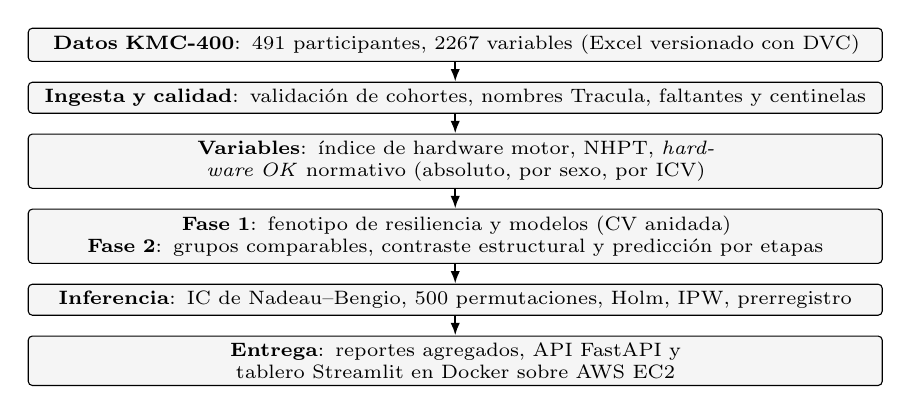
\begin{tikzpicture}[node distance=2.5mm, every node/.style={font=\scriptsize, align=center},
  box/.style={draw, rounded corners=1.5pt, text width=0.88\columnwidth, inner sep=2.5pt, fill=black!4},
  arr/.style={-{Latex[length=1.6mm]}, thick}]
\node[box] (a) {\textbf{Datos KMC-400}: 491 participantes, 2267 variables (Excel versionado con DVC)};
\node[box, below=of a] (b) {\textbf{Ingesta y calidad}: validación de cohortes, nombres Tracula, faltantes y centinelas};
\node[box, below=of b] (c) {\textbf{Variables}: índice de hardware motor, NHPT, \emph{hardware OK} normativo (absoluto, por sexo, por ICV)};
\node[box, below=of c] (d) {\textbf{Fase 1}: fenotipo de resiliencia y modelos (CV anidada)\\
\textbf{Fase 2}: grupos comparables, contraste estructural y predicción por etapas};
\node[box, below=of d] (e) {\textbf{Inferencia}: IC de Nadeau--Bengio, 500 permutaciones, Holm, IPW, prerregistro};
\node[box, below=of e] (f) {\textbf{Entrega}: reportes agregados, API FastAPI y tablero Streamlit en Docker sobre AWS EC2};
\foreach \u/\v in {a/b,b/c,c/d,d/e,e/f} \draw[arr] (\u) -- (\v);
\end{tikzpicture}
\caption{Flujo del proyecto, de los datos crudos al despliegue. Cada etapa es un paso del orquestador \texttt{src/pipeline.py}. Fuente: elaboración propia.}
\label{fig:flujo}
\end{figure}

La Fig.~\ref{fig:flujo} resume el flujo. El análisis avanzó en dos fases: una primera centrada en un fenotipo de resiliencia y una segunda, reorientada con el director y la Fundación tras los resultados de la primera, que parte de grupos comparables y avanza hacia la predicción por etapas.

\subsection{Datos y grupos de análisis}
La base KMC-400 contiene 491 participantes y 2267 variables: los 441 participantes del ensayo reevaluados a los 20 años (228 canguro y 213 tradicional, de 716 vivos al inicio del seguimiento \cite{charpak2017}) y 50 controles nacidos a término. Las variables cubren el contexto social, el embarazo, el nacimiento, la estancia neonatal, la intervención, el seguimiento a 3, 6, 9 y 12 meses de edad corregida, la neuroimagen procesada con FreeSurfer \cite{fischl2012} y Tracula \cite{yendiki2011}, y el NHPT a los 20 años.

Definimos dos grupos comparables. Los \emph{prematuros} son los 209 participantes del ensayo con menos de 1801~g, resonancia estructural y de difusión, y NHPT en ambas manos (112 canguro, 97 tradicional; 168 con buena calidad de imagen). La \emph{referencia} son los controles a término (37 semanas o más y 2500~g o más) sin restricción del crecimiento según Fenton: 38 sujetos, 37 con NHPT y 28 con resonancia. Los 12 controles con restricción del crecimiento se excluyeron por indicación clínica y se conservaron como sensibilidad. La Tabla~\ref{tab:grupos} describe ambos grupos.

\begin{table*}[t]
\caption{Características de los grupos con resonancia: media $\pm$ DE o porcentaje, y g de Hedges (prematuros frente a referencia).}
\label{tab:grupos}
\centering
\footnotesize
\setlength{\tabcolsep}{8pt}
\begin{tabular}{@{}lccc@{}}
\toprule
Variable & Término ($n=28$) & Prematuros ($n=209$) & g [IC 95\,\%] \\
\midrule
Peso al nacer (g) & 3155 $\pm$ 299 & 1558 $\pm$ 233 & $-6{,}59$ [$-7{,}30$; $-5{,}87$] \\
Edad gestacional (sem) & 39,0 $\pm$ 1,0 & 33,1 $\pm$ 2,5 & $-2{,}46$ [$-2{,}91$; $-2{,}00$] \\
Perímetro cefálico (mm)$^a$ & 343,5 $\pm$ 11,2 & 299,2 $\pm$ 17,6 & $-2{,}58$ [$-3{,}13$; $-2{,}04$] \\
Edad de la madre (años) & 24,6 $\pm$ 5,5 & 28,3 $\pm$ 5,7 & $0{,}65$ [$0{,}25$; $1{,}05$] \\
Mujeres (\%) & 53,6 & 58,4 & -- \\
NHPT bimanual (s)$^b$ & 18,86 $\pm$ 1,55 & 19,17 $\pm$ 2,75 & $0{,}12$ [$-0{,}23$; $0{,}47$] \\
\bottomrule
\end{tabular}\\[2pt]
\parbox{0.75\textwidth}{\scriptsize $^a$ Al nacer; disponible en 19 y 166 sujetos. $^b$ Referencia con NHPT, $n=37$. Fuente: elaboración propia a partir de la base KMC-400.}
\end{table*}

\subsection{Preprocesamiento y gobierno de datos}
La ingesta valida tamaños de cohorte, unicidad de identificadores y códigos de grupo, y aborta si algo no coincide. Unificamos 44 columnas de Tracula que el archivo nombraba de forma inconsistente, verificando que cada uno de los 18 tractos quede con sus 18 métricas. Los atípicos no se eliminan por regla automática; se usan estimadores robustos (mediana y MAD escalada). La neuroimagen no se imputa. Las variables clínicas se imputan con MICE \cite{vanbuuren2011} ajustado solo con las filas de entrenamiento de cada partición de validación, después de convertir la escala HOME, que la base codifica como $\pm 1$, a su escala estándar. Las variables con más del 40\,\% de faltantes se excluyen.

El volumen intracraneal (ICV) es a la vez un confusor y un desenlace de la prematurez: es menor en prematuros que en controles (g $=-0{,}61$). Por eso los contrastes entre prematuros y término usan volúmenes absolutos, y el ajuste por ICV se reserva para comparaciones dentro de los prematuros y para el análisis secundario de la Sección~3.6. Los datos clínicos nunca se suben al repositorio: se versionan con DVC en un remoto privado, la fecha de nacimiento se elimina antes de los datos procesados y todos los reportes son agregados.

\subsection{Fase 1: fenotipo de resiliencia}
Construimos un índice de \emph{hardware} motor con 24 medidas de una lista cerrada de 80: volúmenes ajustados por ICV de caudado, putamen, pálido y áreas de Brodmann motoras y somatosensoriales primarias, más FA, difusividad media y radial del tracto corticoespinal, cada una estandarizada de forma robusta. El \emph{software} es el NHPT bimanual estandarizado con el signo invertido. La resiliencia se definió como el residual de una regresión robusta de Huber \cite{huber1964}:
\begin{equation}
r_i = s_i - (\hat\beta_0 + \hat\beta_1 h_i), \qquad \text{resiliente} \iff r_i > 0,
\label{eq:residual}
\end{equation}
donde $s_i$ es el software y $h_i$ el hardware del sujeto $i$ ($n=168$ con buena calidad de imagen). Para predecirla con las 19 variables del formulario clínico (peso, edad gestacional, sexo, fragilidad de Rasch y entorno HOME) se fijó de antemano una regresión logística con regularización L2 y se compararon cuatro alternativas (elastic net, selección con Lasso, Random Forest y gradient boosting), con validación cruzada anidada estratificada \cite{varma2006} y prueba de permutación \cite{ojala2010}.

\subsection{Fase 2: estructura, función y etiqueta normativa}
Siguiendo la reorientación propuesta por el director, comparamos 80 medidas motoras absolutas entre prematuros y referencia con g de Hedges, delta de Cliff, pruebas de Welch y Mann-Whitney, y corrección de Benjamini--Hochberg \cite{benjamini1995}. Con esos tamaños de efecto, la literatura \cite{volpe2009,charpak2017,wilson2017} y la revisión clínica del director, fijamos una lista bilateral de 12 volúmenes que cubre los tres dominios motores: caudado, putamen y pálido, áreas BA4a y BA3b, y tracto corticoespinal. Todos son menores en los prematuros, aunque no todos alcanzan $q_{FDR}<0{,}05$ por separado. La FA y la difusividad radial se excluyeron de la etiqueta porque, como anticipa \cite{groeschel2014}, eran \emph{mejores} en los prematuros que en los controles (FA izquierda $g=+0{,}51$), lo que habría inflado la preservación aparente.

Para cada volumen $k$ y sujeto $i$ calculamos un puntaje normativo anclado a la referencia $\mathcal{R}$:
\begin{equation}
z_{ik} = \frac{x_{ik} - \operatorname{med}_{\mathcal{R}}(x_k)}{1{,}4826\,\operatorname{MAD}_{\mathcal{R}}(x_k)}, \qquad
\bar z_i = \frac{1}{12}\sum_{k=1}^{12} z_{ik}.
\label{eq:norma}
\end{equation}
El promedio $\bar z_i$ se vuelve a estandarizar contra la referencia, porque el promedio de puntajes correlacionados tiene una dispersión menor que uno, y se define \emph{hardware OK} como un puntaje de al menos $-1$ desviación robusta. Como sensibilidades se calcularon la misma etiqueta con normas por sexo, con la referencia completa (incluidos los controles con restricción del crecimiento), con 18 métricas que incluyen FA y difusividad radial, y una versión por conteo que exige que como máximo 2 de los 12 volúmenes estén por debajo de $-1$. Se descartó exigir que los 12 volúmenes superen el umbral a la vez, porque por la probabilidad conjunta de medidas correlacionadas solo 20 de 209 prematuros lo cumplirían, lo que produce un desbalance artificial.

\subsection{Predicción por etapas del desarrollo}
\begin{table}[t]
\caption{Variables clínicas por etapa acumulativa. Nuevas: variables que entran en la etapa; Acum.: total disponible para el modelo.}
\label{tab:variables}
\centering
\footnotesize
\setlength{\tabcolsep}{3pt}
\begin{tabular}{@{}lcc>{\raggedright\arraybackslash}p{0.54\columnwidth}@{}}
\toprule
Etapa & Nuevas & Acum. & Contenido \\
\midrule
Nacimiento & 23 & 23 & Contexto socioeconómico de los padres; antecedentes del embarazo (primiparidad, toxemia, corticoides prenatales, sufrimiento fetal); peso, talla, perímetro cefálico, Apgar, sexo, edad gestacional; índice de fragilidad de Rasch \\
40 semanas & 29 & 52 & Brazo del ensayo y duración en posición canguro; días de hospitalización y de UCI, ventilación, sepsis, enterocolitis, nutrición parenteral; antropometría a las 41 semanas; competencia, apoyo y estrés maternos \\
3 meses & 5 & 57 & Antropometría, INFANIB y tipo de alimentación \\
6 meses & 8 & 65 & Lo anterior a los 6 meses y cocientes de desarrollo de Griffiths \\
9 meses & 5 & 70 & Antropometría, INFANIB y tipo de alimentación \\
12 meses & 19 & 89 & Lo anterior, lactancia materna, entorno HOME, densidad de infecciones, hospitalizaciones y consultas del primer año, ecografía cerebral \\
\bottomrule
\end{tabular}\\[2pt]
\parbox{\columnwidth}{\scriptsize Fuente: elaboración propia.}
\end{table}

Agrupamos 89 variables clínicas en seis etapas acumulativas, de modo que cada modelo solo usa información disponible hasta ese momento (Tabla~\ref{tab:variables}). El mapeo excluye de forma explícita las variables medidas después de la etapa, las versiones incompletas de una misma medida y los identificadores. Los desenlaces fueron el NHPT estandarizado contra la referencia ($n=262$, regresión de Huber) y \emph{hardware OK} ($n=209$, elastic net logístico), con modelos fijados de antemano. En cada etapa comparamos el modelo clínico con un modelo de referencia que solo usa el perímetro cefálico, porque la etiqueta usa volúmenes absolutos y el tamaño de la cabeza predice el tamaño del cerebro.

La evaluación fue una validación cruzada anidada $5\times 5$ con tres particiones internas para hiperparámetros, las mismas particiones en todas las etapas para que las comparaciones fueran pareadas, e imputación ajustada solo con las columnas de cada modelo. Como las particiones repetidas comparten datos, los intervalos de confianza usan la corrección de Nadeau y Bengio \cite{nadeau2003}:
\begin{equation}
\widehat{\operatorname{Var}}(\bar m) = \left(\frac{1}{J} + \frac{n_{\text{prueba}}}{n_{\text{entrenamiento}}}\right) s_m^2,
\label{eq:nb}
\end{equation}
donde $s_m^2$ es la varianza de la métrica entre las $J=25$ particiones. Un modelo \emph{supera al azar} si su p de permutación (500 permutaciones) ajustado por Holm \cite{holm1979} es menor que 0,05 y el límite inferior del intervalo excluye el azar. Solo para los modelos que superan al azar se calcula la importancia media $|\text{SHAP}|$ por variable \cite{lundberg2017}, con un explicador lineal cuya referencia es el vector de medias de entrenamiento, de modo que el paquete exportado no guarda filas de sujetos. Como sensibilidades se usaron Random Forest y gradient boosting, imputación por mediana, la submuestra con buena calidad de imagen y pesos de probabilidad inversa (IPW) por disponibilidad de resonancia, que corrigen la posible selección de los 51 prematuros sin imagen.

\subsection{Análisis secundario: tamaño frente a calidad}
Para saber si la señal sobre \emph{hardware OK} refleja el tamaño o la calidad de la estructura, registramos antes de correrlo un análisis con una etiqueta ajustada por ICV: para cada volumen se ajustó $\text{volumen} \sim \text{ICV} + \text{sexo}$ por mínimos cuadrados en la referencia, y la Ecuación~\eqref{eq:norma} se aplicó a los residuales. La regla de interpretación fijada de antemano fue: \emph{calidad} si el modelo clínico supera al azar y a los modelos de solo perímetro y de perímetro más sexo; \emph{intermedio} si supera al azar pero no a ambas referencias; y \emph{tamaño} si no supera al azar.

\subsection{Entorno de implementación y despliegue}
El código está en Python 3.12 con scikit-learn, gestionado con uv. Un orquestador ejecuta los ocho pasos del flujo (ingesta, hardware motor, resiliencia, \emph{hardware OK}, imputación, IPW, modelos por etapa y análisis por ICV) y en modo estricto falla si falta alguno. La calidad se asegura con integración continua en GitHub Actions (ruff, mypy y 190 pruebas con datos reales en local), revisión obligatoria de cada cambio y un registro de 42 decisiones con su justificación. Los experimentos se registran con MLflow. La entrega es una API en FastAPI y un tablero en Streamlit, en contenedores Docker sobre una instancia EC2 de AWS: el tablero muestra solo resultados poblacionales y es público, mientras que la API y el acceso administrativo están restringidos a una dirección autorizada. Los modelos se montan como volumen de solo lectura y no forman parte de las imágenes.

% =====================================================================
\section{Resultados}

\subsection{Estructura y función: una disociación a nivel de grupo}
De las 65 métricas del atlas principal, 32 difieren entre prematuros y referencia ($q_{FDR}<0{,}05$). La Fig.~\ref{fig:estructura}a muestra los 12 volúmenes de la etiqueta: todos son menores en los prematuros, con efectos grandes en el caudado izquierdo ($g=-0{,}90$), el tracto corticoespinal derecho ($-0{,}87$), el caudado derecho ($-0{,}85$) y el pálido derecho ($-0{,}83$). En cambio, el NHPT casi no difiere (Fig.~\ref{fig:estructura}b): 19,17~s en prematuros frente a 18,86~s en la referencia ($g=0{,}12$; IC 95\,\% $[-0{,}23;\,0{,}47]$), sin diferencia entre canguro y tradicional. Incluso los controles son más lentos que las normas de Mathiowetz: el 97\,\% supera la media normativa, por lo que el NHPT se estandarizó contra la referencia local.

\begin{figure*}[t]
\centering
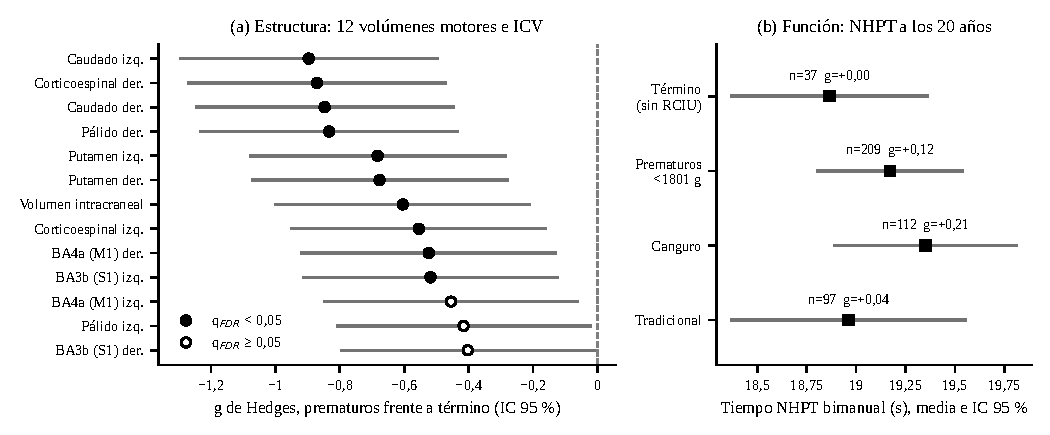
\includegraphics[width=0.92\textwidth]{figuras/fig_estructura_nhpt.pdf}
\caption{(a) Diferencia de los 12 volúmenes motores de la etiqueta y del volumen intracraneal entre prematuros ($n=209$) y controles a término sin restricción del crecimiento ($n=28$); puntos rellenos: $q_{FDR}<0{,}05$. (b) Tiempo bimanual en el NHPT por grupo; g de Hedges frente a la referencia. Fuente: elaboración propia.}
\label{fig:estructura}
\end{figure*}

Dentro de los prematuros, la estructura sí se relaciona con la función, aunque débilmente: el puntaje normativo de los 12 volúmenes tiene una correlación parcial, ajustada por sexo, de $r=-0{,}26$ (IC 95\,\% $[-0{,}39;\,-0{,}13]$) con el tiempo en el NHPT, es decir, más volumen se asocia con menos tiempo.

\subsection{Fase 1: la resiliencia no es predecible}
La relación entre hardware y software fue débil (pendiente de Huber 0,31; $R^2=0{,}022$ en mínimos cuadrados), con 90 de 168 participantes clasificados como resilientes. Con las 19 variables del formulario, ningún modelo superó al azar (Tabla~\ref{tab:modelos}): el modelo base obtuvo ROC-AUC $0{,}531\pm 0{,}081$ y el mejor, gradient boosting, $0{,}555\pm 0{,}054$, dentro del margen del 95\,\% de un clasificador aleatorio con $n=168$ ($0{,}50\pm 0{,}09$ \cite{hanley1982}). La prueba de permutación del modelo exportado dio $p=0{,}353$.

\begin{table}[t]
\caption{Resumen de la capacidad predictiva por desenlace.}
\label{tab:modelos}
\centering
\footnotesize
\setlength{\tabcolsep}{3pt}
\begin{tabular}{@{}lccc@{}}
\toprule
Desenlace & $n$ & Métrica & Resultado \\
\midrule
Resiliencia (modelo base) & 168 & ROC-AUC & $0{,}531 \pm 0{,}081$ \\
Resiliencia (mejor modelo) & 168 & ROC-AUC & $0{,}555 \pm 0{,}054$ \\
NHPT, 6 etapas & 262 & $R^2$ & $-0{,}076$ a $-0{,}046$ \\
\emph{Hardware OK}, nacimiento & 209 & ROC-AUC & $0{,}703$ [$0{,}631$; $0{,}775$] \\
\emph{Hardware OK}, 12 meses & 209 & ROC-AUC & $0{,}771$ [$0{,}690$; $0{,}853$] \\
\emph{Hardware OK}, ajuste ICV & 209 & ROC-AUC & $0{,}635$ a $0{,}668$ \\
\bottomrule
\end{tabular}\\[2pt]
\parbox{\columnwidth}{\scriptsize Resiliencia: media $\pm$ DE entre particiones. Demás filas: media e IC 95\,\% de Nadeau--Bengio, o rango entre etapas. Fuente: elaboración propia.}
\end{table}

\subsection{Fase 2: predicción por etapas}
\emph{Hardware OK} clasificó a 98 de 209 prematuros (46,9\,\%) como estructuralmente preservados (84 de 168 con buena calidad de imagen). Las variantes dieron prevalencias similares: 93 con la referencia completa, 79 con normas por sexo, 99 con 18 métricas y 77 por conteo, por lo que la etiqueta conserva un balance de clases cercano al 40--50\,\% en todas. La Tabla~\ref{tab:etapas} y la Fig.~\ref{fig:etapas} muestran los resultados por etapa. El NHPT no fue predecible en ninguna: el $R^2$ fuera de muestra fue negativo en todas las etapas y modelos, con todos los intervalos incluyendo cero (Fig.~\ref{fig:etapas}c). \emph{Hardware OK} superó al azar en las seis etapas (p de permutación 0,002; p de Holm 0,024), con un AUC de 0,70 al nacer que sube a 0,77 a los 12 meses. El salto más grande ocurrió entre las 40 semanas y los 3 meses ($+0{,}060$; IC $[0{,}014;\,0{,}107]$), cuando entra el perímetro cefálico de esa edad.

\begin{table}[t]
\caption{ROC-AUC fuera de muestra por etapa del desarrollo. Clín.: variables clínicas; PC: solo perímetro cefálico; PC+S: perímetro y sexo.}
\label{tab:etapas}
\centering
\footnotesize
\setlength{\tabcolsep}{3.5pt}
\begin{tabular}{@{}lccccc@{}}
\toprule
& \multicolumn{2}{c}{\emph{Hardware OK}} & \multicolumn{3}{c}{Ajustado por ICV} \\
\cmidrule(lr){2-3}\cmidrule(lr){4-6}
Etapa & Clín. & PC & Clín. & PC & PC+S \\
\midrule
Nacimiento & 0,703 & 0,611 & 0,635 & 0,618 & 0,607 \\
40 semanas & 0,685 & 0,617 & 0,668 & 0,595 & 0,585 \\
3 meses & 0,746 & 0,712 & 0,652 & 0,608 & 0,595 \\
6 meses & 0,756 & 0,736 & 0,652 & 0,619 & 0,612 \\
9 meses & 0,768 & 0,746 & 0,651 & 0,628 & 0,619 \\
12 meses & 0,771 & 0,739 & 0,637 & 0,623 & 0,614 \\
\bottomrule
\end{tabular}\\[2pt]
\parbox{\columnwidth}{\scriptsize $n=209$; validación cruzada anidada $5\times5$. Fuente: elaboración propia.}
\end{table}

\begin{figure*}[t]
\centering
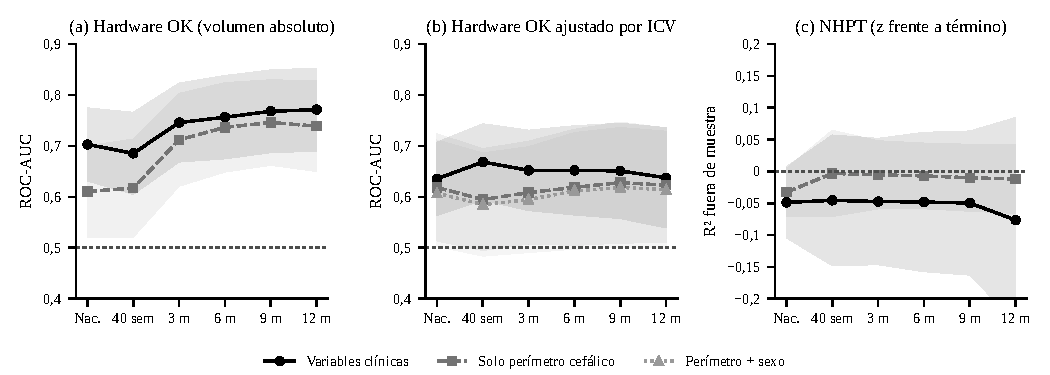
\includegraphics[width=0.92\textwidth]{figuras/fig_etapas.pdf}
\caption{Desempeño fuera de muestra por etapa acumulativa, con IC 95\,\% de Nadeau--Bengio (bandas). (a) \emph{Hardware OK} con volúmenes absolutos. (b) \emph{Hardware OK} ajustado por volumen intracraneal y sexo. (c) NHPT estandarizado contra la referencia. La línea punteada marca el azar. Fuente: elaboración propia.}
\label{fig:etapas}
\end{figure*}

Sin embargo, el modelo de solo perímetro cefálico explica casi todo ese desempeño. Su diferencia con el modelo clínico solo fue significativa al nacer ($+0{,}092$; IC $[0{,}016;\,0{,}168]$, sin ajuste por multiplicidad), y un análisis exploratorio mostró que esa ventaja era el sexo: con perímetro y sexo el AUC al nacer fue 0,716, por encima del modelo clínico completo, y ninguna variable clínica adicional aportó de forma significativa (24 pruebas, p de Holm $\ge 0{,}95$). El sexo aporta porque la etiqueta usa normas comunes y los hombres tienen volúmenes mayores: con normas por sexo, el AUC baja a 0,58--0,69 y el sexo deja de aportar. Las sensibilidades con otras familias de modelos, imputación por mediana, IPW (pesos entre 0,85 y 1,42; diferencia de medias estandarizada máxima de 0,060 sin pesos y 0,009 con pesos) y la submuestra con buena calidad de imagen mantuvieron el patrón. Los pesos son casi planos porque los 51 prematuros sin resonancia se parecen a los que sí la tienen: no difieren en las variables del nacimiento, el nivel socioeconómico, la fragilidad ni el entorno HOME, y solo difieren en el estado civil de la madre ($p=0{,}012$).

La importancia media $|\text{SHAP}|$ confirma esta lectura. Al nacer, el sexo domina con amplitud (0,58 en log-odds, más del doble que la siguiente variable), seguido de antecedentes del embarazo como la primiparidad, con dirección negativa, y el perímetro cefálico. A los 12 meses, el perímetro cefálico de los 6 meses (0,35) casi iguala al sexo (0,37), y la duración en posición canguro y la lactancia materna a los 12 meses aparecen con peso menor y dirección positiva. Estas importancias describen el modelo, no efectos causales, y ninguna de esas variables aportó de forma significativa por encima del perímetro y el sexo.

\subsection{Tamaño frente a calidad}
Al descontar el ICV y el sexo, la etiqueta clasificó a 133 de 209 prematuros como preservados, y los modelos de solo perímetro y de perímetro más sexo cayeron al borde del azar (AUC 0,58--0,63; Fig.~\ref{fig:etapas}b). El modelo clínico conservó una señal modesta que supera al azar en las seis etapas (AUC 0,64--0,67; p de Holm 0,036), estable desde las 40 semanas. Su ventaja sobre las referencias fue positiva en todas las etapas ($+0{,}015$ a $+0{,}074$ frente a solo perímetro), pero ningún intervalo excluyó cero. Según la regla prerregistrada, el resultado es \emph{intermedio} en las seis etapas.

\subsection{Sistema desplegado}
El tablero público presenta los grupos comparables, el NHPT por grupo, el contraste estructural, la calibración de \emph{hardware OK} y las curvas por etapa con sus sensibilidades, incluido el análisis por ICV, leyendo solo reportes agregados. El formulario de predicción individual se mantiene como demostración técnica, con una advertencia explícita de que el modelo no supera al azar. En la instancia de AWS, una prueba de humo verificó que la API reporta los artefactos disponibles y responde a una predicción con valores sintéticos.

% =====================================================================
\section{Discusión}

\subsection{Interpretación}
El hallazgo central es una disociación a nivel de grupo: los prematuros tienen volúmenes motores claramente menores, pero su destreza manual a los 20 años es comparable a la de los controles. Esto es coherente con la observación clínica que motivó el proyecto y sugiere que, para la mayoría, la función motora fina se preserva pese a la huella anatómica. Dentro de los prematuros la estructura se asocia con la función ($r=-0{,}26$), en la misma dirección que la relación entre caudado y NHPT reportada en \cite{charpak2017}, pero explica poco de su variabilidad.

Que el NHPT no sea predecible con información temprana tiene varias explicaciones no excluyentes: el tamaño de la muestra, la confiabilidad test-retest moderada de la prueba \cite{mathiowetz1985}, que limita la varianza explicable, y la posibilidad de que lo que determina la destreza a los 20 años ocurra después del primer año. El fenotipo de resiliencia hereda ese ruido: como el hardware explica el 2\,\% del software, el residual de la Ecuación~\eqref{eq:residual} refleja sobre todo el NHPT, y no sorprende que tampoco sea predecible.

La estructura, en cambio, sí es predecible, pero sobre todo por su tamaño. Que el perímetro cefálico anticipe el volumen cerebral a los 20 años es esperable, y es coherente con el papel predictivo del perímetro al final del primer año que Charpak et al. señalan en esta cohorte, donde se asocia con el cociente intelectual a los 20 años \cite{charpak2017}. El análisis por ICV muestra que, una vez descontado el tamaño, queda una señal de calidad estructural presente desde las 40 semanas, que no podemos atribuir a variables clínicas específicas con 209 sujetos. La discusión sobre qué etiqueta usar (normas comunes, por sexo o ajustadas por ICV) es una decisión sobre la definición del desenlace y no sobre el modelado; proponemos reportar la etiqueta absoluta como principal y la ajustada por ICV como el análisis que separa tamaño de calidad.

\subsection{Aportes y aplicaciones}
Frente a la literatura de aprendizaje automático en prematuros, que reporta desempeños altos con muestras pequeñas y sin validación externa \cite{baker2023}, este trabajo muestra lo que queda cuando la evaluación se hace con validación anidada, permutaciones, corrección por multiplicidad y modelos de referencia simples: un resultado nulo robusto para la función y una señal moderada, explicada sobre todo por el crecimiento cefálico, para la estructura. Ese contraste es en sí una contribución metodológica. En la práctica, el resultado respalda el seguimiento del perímetro cefálico como marcador temprano de la estructura cerebral adulta, y el tablero permite a la Fundación consultar los resultados poblacionales sin exponer datos individuales.

\subsection{Limitaciones}
La referencia con resonancia es pequeña (28 sujetos), por lo que las normas, y en especial el ajuste por ICV y sexo, son inestables: con la referencia completa la prevalencia de \emph{hardware OK} ajustado pasa de 133 a 164 de 209, y por eso las conclusiones se apoyan en el patrón y no en el nivel. El estudio usa una sola cohorte, sin validación externa. Los pesos IPW solo corrigen la selección por las variables observadas y no la pérdida de seguimiento desde el nacimiento (716 a 441), para la que no hay datos de los perdidos. La exclusión por calidad de imagen no fue pareja entre brazos: se conservó el 84\,\% del grupo canguro y el 76\,\% del tradicional. Finalmente, todos los resultados son asociaciones y no efectos causales.

% =====================================================================
\section{Conclusiones y trabajo futuro}

Los adultos nacidos con menos de 1801~g en el ensayo del MMC tienen una estructura motora cerebral claramente reducida, pero una destreza manual comparable a la de los controles a término. Con la información clínica del primer año no es posible predecir esa destreza ni un fenotipo de resiliencia basado en la disociación entre estructura y función. La preservación de la estructura motora sí es predecible desde el nacimiento (AUC 0,70) hasta los 12 meses (0,77), pero esa capacidad se debe sobre todo al perímetro cefálico y al sexo; descontado el tamaño, persiste una señal modesta de calidad estructural (AUC $\approx 0{,}65$). Reportamos estos resultados nulos y parciales como hallazgos, sustentados en una evaluación rigurosa y en un sistema reproducible y desplegado.

Como trabajo futuro proponemos: ampliar el grupo de referencia a término con más controles con resonancia, lo que estabilizaría las normas y el ajuste por ICV; estudiar desenlaces motores menos ruidosos o compuestos, y variables posteriores al primer año; estimar el efecto causal del MMC con estimadores doblemente robustos y pesos por la pérdida de seguimiento, lo que requiere los datos de los participantes perdidos; e identificar subgrupos de participantes con patrones distintos de estructura y función, como plantea la propuesta original.

\section*{Agradecimientos}
Agradecemos a la Fundación Canguro por el acceso a la cohorte KMC-400 y por resolver las preguntas clínicas del análisis, y al profesor Tiberio por la dirección del proyecto. Agradecemos también a la Universidad de los Andes y a la Maestría en Inteligencia Artificial por el espacio académico y la formación que hicieron posible este trabajo, y a los participantes del estudio y sus familias, cuyo compromiso durante dos décadas de seguimiento sostiene todo lo aquí reportado.

\newpage
\begin{thebibliography}{99}
\bibitem{darmstadt2023} G. L. Darmstadt, N. H. Al Jaifi, S. Arif, R. Bahl, M. Blennow, V. Cavallera \emph{et al.}, ``New World Health Organization recommendations for care of preterm or low birth weight infants: health policy,'' \emph{EClinicalMedicine}, vol. 63, art. 102155, Sep. 2023, doi: 10.1016/j.eclinm.2023.102155.
\bibitem{charpak2017} N. Charpak, R. Tessier, J. G. Ruiz, J. T. Hernandez, F. Uriza, J. Villegas \emph{et al.}, ``Twenty-year follow-up of kangaroo mother care versus traditional care,'' \emph{Pediatrics}, vol. 139, no. 1, art. e20162063, Jan. 2017, doi: 10.1542/peds.2016-2063.
\bibitem{charpak2022} N. Charpak, R. Tessier, J. G. Ruiz, F. Uriza, J. T. Hernandez, D. Cortes, and A. Montealegre-Pomar, ``Kangaroo mother care had a protective effect on the volume of brain structures in young adults born preterm,'' \emph{Acta Paediatr.}, vol. 111, no. 5, pp. 1004--1014, May 2022, doi: 10.1111/apa.16265.
\bibitem{volpe2009} J. J. Volpe, ``Brain injury in premature infants: a complex amalgam of destructive and developmental disturbances,'' \emph{Lancet Neurol.}, vol. 8, no. 1, pp. 110--124, Jan. 2009, doi: 10.1016/S1474-4422(08)70294-1.
\bibitem{nosarti2014} C. Nosarti, K. W. Nam, M. Walshe, R. M. Murray, M. Cuddy, L. Rifkin, and M. P. G. Allin, ``Preterm birth and structural brain alterations in early adulthood,'' \emph{NeuroImage: Clin.}, vol. 6, pp. 180--191, 2014, doi: 10.1016/j.nicl.2014.08.005.
\bibitem{groeschel2014} S. Groeschel, J.-D. Tournier, G. B. Northam, T. Baldeweg, J. Wyatt, B. Vollmer, and A. Connelly, ``Identification and interpretation of microstructural abnormalities in motor pathways in adolescents born preterm,'' \emph{NeuroImage}, vol. 87, pp. 209--219, Feb. 2014, doi: 10.1016/j.neuroimage.2013.10.034.
\bibitem{salazar2026} M. Salazar Iglesias and J. A. Pineda, ``Atención y función ejecutiva en jóvenes nacidos prematuros: efecto del Método Madre Canguro 20 años después,'' Proyecto final, Maestría en Inteligencia Artificial, Universidad de los Andes, Bogotá, Colombia, 2026.
\bibitem{wilson2017} P. H. Wilson, B. Smits-Engelsman, K. Caeyenberghs, B. Steenbergen, D. Sugden, J. Clark, N. Mumford, and R. Blank, ``Cognitive and neuroimaging findings in developmental coordination disorder: new insights from a systematic review of recent research,'' \emph{Dev. Med. Child Neurol.}, vol. 59, no. 11, pp. 1117--1129, Nov. 2017, doi: 10.1111/dmcn.13530.
\bibitem{mathiowetz1985} V. Mathiowetz, K. Weber, N. Kashman, and G. Volland, ``Adult norms for the Nine Hole Peg Test of finger dexterity,'' \emph{Occup. Ther. J. Res.}, vol. 5, no. 1, pp. 24--38, Jan. 1985, doi: 10.1177/153944928500500102.
\bibitem{baker2023} S. Baker and Y. Kandasamy, ``Machine learning for understanding and predicting neurodevelopmental outcomes in premature infants: a systematic review,'' \emph{Pediatr. Res.}, vol. 93, no. 2, pp. 293--299, Jan. 2023, doi: 10.1038/s41390-022-02120-w.
\bibitem{marquand2016} A. F. Marquand, I. Rezek, J. Buitelaar, and C. F. Beckmann, ``Understanding heterogeneity in clinical cohorts using normative models: beyond case-control studies,'' \emph{Biol. Psychiatry}, vol. 80, no. 7, pp. 552--561, Oct. 2016, doi: 10.1016/j.biopsych.2015.12.023.
\bibitem{fischl2012} B. Fischl, ``FreeSurfer,'' \emph{NeuroImage}, vol. 62, no. 2, pp. 774--781, Aug. 2012, doi: 10.1016/j.neuroimage.2012.01.021.
\bibitem{yendiki2011} A. Yendiki, P. Panneck, P. Srinivasan, A. Stevens, L. Zöllei, J. Augustinack \emph{et al.}, ``Automated probabilistic reconstruction of white-matter pathways in health and disease using an atlas of the underlying anatomy,'' \emph{Front. Neuroinform.}, vol. 5, art. 23, Oct. 2011, doi: 10.3389/fninf.2011.00023.
\bibitem{vanbuuren2011} S. van Buuren and K. Groothuis-Oudshoorn, ``mice: Multivariate imputation by chained equations in R,'' \emph{J. Stat. Softw.}, vol. 45, no. 3, pp. 1--67, Dec. 2011, doi: 10.18637/jss.v045.i03.
\bibitem{huber1964} P. J. Huber, ``Robust estimation of a location parameter,'' \emph{Ann. Math. Statist.}, vol. 35, no. 1, pp. 73--101, Mar. 1964, doi: 10.1214/aoms/1177703732.
\bibitem{varma2006} S. Varma and R. Simon, ``Bias in error estimation when using cross-validation for model selection,'' \emph{BMC Bioinformatics}, vol. 7, art. 91, Feb. 2006, doi: 10.1186/1471-2105-7-91.
\bibitem{ojala2010} M. Ojala and G. C. Garriga, ``Permutation tests for studying classifier performance,'' \emph{J. Mach. Learn. Res.}, vol. 11, pp. 1833--1863, Jun. 2010.
\bibitem{benjamini1995} Y. Benjamini and Y. Hochberg, ``Controlling the false discovery rate: a practical and powerful approach to multiple testing,'' \emph{J. R. Stat. Soc. Ser. B (Methodol.)}, vol. 57, no. 1, pp. 289--300, Jan. 1995.
\bibitem{nadeau2003} C. Nadeau and Y. Bengio, ``Inference for the generalization error,'' \emph{Mach. Learn.}, vol. 52, no. 3, pp. 239--281, Sep. 2003, doi: 10.1023/A:1024068626366.
\bibitem{holm1979} S. Holm, ``A simple sequentially rejective multiple test procedure,'' \emph{Scand. J. Statist.}, vol. 6, no. 2, pp. 65--70, 1979.
\bibitem{lundberg2017} S. M. Lundberg and S.-I. Lee, ``A unified approach to interpreting model predictions,'' in \emph{Advances in Neural Information Processing Systems}, vol. 30, 2017, pp. 4765--4774.
\bibitem{hanley1982} J. A. Hanley and B. J. McNeil, ``The meaning and use of the area under a receiver operating characteristic (ROC) curve,'' \emph{Radiology}, vol. 143, no. 1, pp. 29--36, Apr. 1982, doi: 10.1148/radiology.143.1.7063747.
\end{thebibliography}

\end{document}
